\documentclass{article}
    
    \usepackage{graphicx} % Used to insert images
    \usepackage{adjustbox} % Used to constrain images to a maximum size 
    \usepackage{color} % Allow colors to be defined
    \usepackage{enumerate} % Needed for markdown enumerations to work
    \usepackage{geometry} % Used to adjust the document margins
    \usepackage{amsmath} % Equations
    \usepackage{amssymb} % Equations
    \usepackage{eurosym} % defines \euro
    \usepackage[mathletters]{ucs} % Extended unicode (utf-8) support
    \usepackage[utf8x]{inputenc} % Allow utf-8 characters in the tex document
    \usepackage{fancyvrb} % verbatim replacement that allows latex
    \usepackage{grffile} % extends the file name processing of package graphics 
                         % to support a larger range 
    % The hyperref package gives us a pdf with properly built
    % internal navigation ('pdf bookmarks' for the table of contents,
    % internal cross-reference links, web links for URLs, etc.)
    \usepackage{hyperref}
    \usepackage{longtable} % longtable support required by pandoc >1.10
    \usepackage{booktabs}  % table support for pandoc > 1.12.2
    \usepackage{indentfirst}
    \usepackage{floatrow}
    \usepackage{relsize}
    \usepackage{multirow}
        
    \newcommand\perm[2]{{}_{#1}P_{#2}}%
    \newcommand\todo[1]{\textbf{TODO: #1}}% 
    \newcommand\numberthis{\addtocounter{equation}{1}\tag{\theequation}}
    \newcommand\seteq{\mathrel{\overset{\makebox[0pt]{\mbox{\normalfont\small\sffamily set}}}{=}}}
    \newcommand\mfrac[2]{\left(\dfrac{#1}{#2}\right)}
    \newcommand\lint{\mathlarger{\int}}
    \newcommand\lsum{\mathlarger{\sum}}
    \newcommand\lprod{\mathlarger{\prod}}
    \newcommand\myskip[1]{\addtocounter{enumi}{#1}}
    
    \title{Homework 14}
    \author{Roly Vicar\'ia \\ STAT414 Spring 2016}
    
\begin{document}
    
    \maketitle
    
    \textbf{Section 5.5}
    \begin{enumerate}
      \myskip{1}
      
      %2
      \item
	$X \sim N(50,36)$
	\begin{figure}[h!]
	  \centering
	  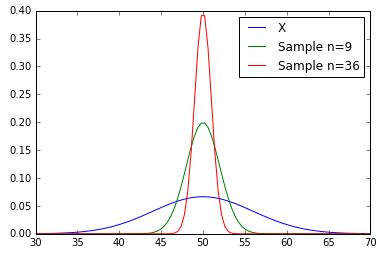
\includegraphics[scale=.8]{./images/2_plotSampleDistributions.png}
	  % 2_plotSampleDistributions.png: 384x257 pixel, 96dpi, 10.16x6.80 cm, bb=0 0 288 193
	\end{figure}
      
      %3
      \item
	\begin{enumerate}
	 %a
	 \item 
	  $E(\bar{X}) = \mu = 46.58$, \\
	  $Var(\bar{X}) = \dfrac{\sigma^2}{n} = \dfrac{40.96}{16} = 2.56$
	  
	 %b
	 \item
	  \begin{align*}
	   P(44.42 \le \bar{X} \le 48.98) &= 
	    P\left(\dfrac{44.42 - 46.58}{\sqrt{2.56}} \le \dfrac{\bar{X} - 46.58}{\sqrt{2.56}} \le 
	      \dfrac{48.98 - 46.58}{\sqrt{2.56}}\right) \\
	    &= P(-1.35 \le Z \le 1.5) \\
	    &= \Phi(1.5) - \Phi(-1.35) \\
	    &= 0.9332 - 0.0885 \\
	    &= 0.8447
	  \end{align*}
	\end{enumerate}
      \myskip{1}
      
      \newpage
      %5
      \item
	\begin{enumerate}
	 %a
	 \item
	  $X \sim N(8.78,0.16)$
	  \begin{figure}[h!]
	    \centering
	    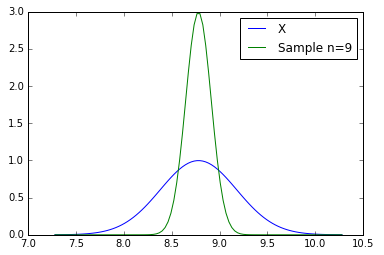
\includegraphics[scale=.7]{./images/5a_plotSampleDistribution.png}
	    % 5a_plotSampleDistribution.png: 384x255 pixel, 96dpi, 10.16x6.75 cm, bb=0 0 288 191
	  \end{figure}
	 
	 %b
	 \item
	  To find $a$ and $b$, such that $P(a \le S^2 \le b) = 0.90$, we use the fact that 
	  $\dfrac{(n-1)S^2}{\sigma^2}$ is $\chi^2(8)$, therefore, we restate the question as 
	  $P\left(\dfrac{8a}{0.16} \le \dfrac{8 S^2}{0.16} \le \dfrac{8b}{0.16}\right) = 0.90$.
	  
	  This is the same as $P\left(\dfrac{8 S^2}{0.16} \le \dfrac{8b}{0.16}\right) 
	    - P\left(\dfrac{8 S^2}{0.16} \le \dfrac{8a}{0.16}\right) = 0.90$
	    
	  From Table IV in the book, we can see that $P\left(\dfrac{8 S^2}{0.16} \le 15.51\right) 
	    - P\left(\dfrac{8 S^2}{0.16} \le 2.733\right) = 0.90$.
	    
	  Solving for $a = \dfrac{2.733 \cdot 0.16}{8} = 0.5466$ and 
	  $b = \dfrac{15.51 \cdot 0.16}{8} = 0.3102$	  
	\end{enumerate}
      \myskip{1}
      
      %7
      \item
	We start by defining $Y = X_1 + X_2 + X_3$, where $X_i \sim N(1.18, 0.07^2)$. Therefore,
	$Y \sim N(3.54, 0.0147)$. We are also given $W \sim N(3.22, 0.09^2)$. We can compute that
	$Y-W \sim N(0.32, 0.0228)$. 
	
	We are asked to find the $P(Y > W) = P(Y-W > 0) 
	  = P\left(\dfrac{Y-W - 0.32}{\sqrt{0.0228}} > \dfrac{0-0.32}{\sqrt{0.0228}}\right)
	  = P(Z > -2.12) = P(Z < 2.12) = 0.9830$
      
      %8
      \item
	We are given that $X \sim N(184.09,39.37)$ and $Y \sim N(171.93,50.88)$. We can compute that
	$X - Y \sim N(12.16, 90.25)$. Therefore, $P(X > Y) = P(X - Y > 0) 
	  = P\left(Z > \dfrac{-12.16}{\sqrt{90.25}}\right) = P(Z > -1.28) = P(Z < 1.28) = 0.8997$
      \myskip{1}
      
      %10
      \item
	We are given that we have $n$ light bulbs, each one follows a normal distribution, $N(800, 100^2)$.
	We want the sum of the lifetime of the $n$ lightbulbs to be greater than 10,000 hours with 
	probability 0.90. In other words, we are looking for $n$, such that $P(Y > 10000) = 0.90)$, 
	where $Y = X_1 + X_2 + \cdots + X_n$. 
	
	We know that $Y \sim N(800n, 100^2n)$. Therefore, 
	\begin{align*}
	 P(Y > 10000) &= P\left(\dfrac{Y - 800n}{\sqrt{100^2n}} > \dfrac{10000 - 800n}{\sqrt{100^2n}}\right) \\
	  &= P\left(Z > \dfrac{10000 - 800n}{\sqrt{100^2n}}\right) = 0.90
	\end{align*}
	
	We can rexpress that last equality as $P\left(Z < -\dfrac{10000 - 800n}{\sqrt{100^2n}}\right) = 0.90$.
	From table Va in the book, we find that $P(Z < 1.29) \approx 0.90$. 
	
	Solving the following for $n$, 
	
	\begin{align*}
	 1.29 &= -\dfrac{10000 - 800n}{\sqrt{100^2n}}
	\end{align*}
	
	We get $n = 13.08$. Rounding up, $n=14$.
      \myskip{4}
      
      %15
      \item
	\begin{enumerate}
	 %a
	 \item
	  $t_{0.01}(17) = 2.567$
	 
	 %b
	 \item
	  $t_{0.95}(17) = -1.740$
	 
	 %c
	 \item
	  $P(-1.740 \le T \le 1.740) = 0.90$
	\end{enumerate}
      
      %16
      \item
	$T \sim t(8)$
	\begin{enumerate}
	 %a
	 \item 
	  $P(-t_{0.025} \le T \le t_{0.025}) = 0.95$ \\
	  $t_{0.025} = 2.306$
	 
	 %b
	 \item
	  $$-t_{0.025} \le T \le t_{0.025}$$
	  $$-t_{0.025} \le \dfrac{\bar{X} - \mu}{S/\sqrt{n}} \le t_{0.025}$$
	  $$-t_{0.025}\dfrac{S}{\sqrt{n}} \le \bar{X} - \mu \le t_{0.025}\dfrac{S}{\sqrt{n}}$$
	  $$-\bar{X} - t_{0.025}\dfrac{S}{\sqrt{n}} \le -\mu \le -\bar{X} + t_{0.025}\dfrac{S}{\sqrt{n}}$$
	  $$\bar{X} - t_{0.025}\dfrac{S}{\sqrt{n}} \le \mu \le \bar{X} + t_{0.025}\dfrac{S}{\sqrt{n}}$$

	\end{enumerate}
    \end{enumerate}
    
    \textbf{Section 5.6}
    \begin{enumerate}
     %1
     \item 
      $P(1/2 \le \bar{X} \le 2/3) = P\left(\dfrac{1/2 - 1/2}{1/12} \le Z \le \dfrac{2/3 - 1/2}{1/12}\right) 
       = P(0 \le Z \le 2) \\ = \Phi(2) - \Phi(0) = 0.9772 - 0.5 = 0.4772$
     \myskip{1}
     
     %3
     \item
      $P(2.5 \le \bar{X} \le 4) = P\left(\dfrac{2.5 - 3}{.5} \le Z \le \dfrac{4 - 3}{.5}\right)
	= P(-1 \le Z \le 2) \\ = \Phi(2) - \Phi(-1) = 0.9772 - 0.1587 = 0.8185$
     \myskip{1}
     
     %5
     \item
      \begin{enumerate}
       %a
       \item 
	$Y \sim \chi^2(18)$
	
       %b
       \item
	To approximate $P(Y \le 9.390)$ using the central limit theorem, we first observe that $Y$ has
	a mean $\mu = r = 18$ and a variance $\sigma^2 = 2r = 36$. Therefore,
	$$P(Y \le 9.390) \approx P\left(Z \le \dfrac{9.390 - 18}{6/\sqrt{18}}\right) = P(Z \le -6.088)
	  \approx 0$$
	  
	To approximate $P(Y \le 34.80)$, we do the same as above and get,
	$$P(Y \le 34.80) \approx P\left(Z \le \dfrac{34.80 - 18}{6/\sqrt{18}}\right) = P(Z \le 11.879)
	  \approx 1$$
	  
	These approximations are fair considering that the exact values are $0.05$ and $1$. Since 
	$\chi^2$ is a skewed distribution, we require more samples for better approximations.
      \end{enumerate}
     
     %6
     \item
      \begin{enumerate}
       %a
       \item
	\begin{align*}
	 \mu = E(X) &= \lint_0^2{x \left(1 - \dfrac{x}{2}\right)dx}  \\
	  &= \lint_0^2 { x dx} - \dfrac{1}{2}\lint_0^2{x^2 dx} \\
	  &= \dfrac{x^2}{2}\Big|_0^2 - \dfrac{x^3}{6}\Big|_0^2 \\
	  &= 2 - \dfrac{8}{6} \\
	  &= \dfrac{2}{3}
	\end{align*}
	
	\begin{align*}
	 E(X^2) &= \lint_0^2{x^2 \left(1 - \dfrac{x}{2}\right)dx} \\
	  &= \lint_0^2{x^2 dx} - \dfrac{1}{2}\lint_0^2 {x^3 dx} \\
	  &= \dfrac{x^3}{3}\Big|_0^2 - \dfrac{x^4}{8}\Big|_0^2 \\
	  &= \dfrac{8}{3} - 2 \\
	  &= \dfrac{2}{3}
	\end{align*}
	
	\begin{align*}
	 Var(X) &= E(X^2) - [E(X)]^2 \\
	  &= \dfrac{2}{3} - \mfrac{2}{3}^2 \\
	  &= \dfrac{2}{9}
	\end{align*}
       
       %b
       \item
	\begin{align*}
	 P(2/3 \le \bar{X} \le 5/6) &\approx P\left(\dfrac{2/3 - 2/3}{\sqrt{2/9}/\sqrt{18}} \le Z
	      \le \dfrac{5/6 - 2/3}{\sqrt{2/9}/\sqrt{18}}\right) \\
	  &= P(0 \le Z \le 1.5) \\
	  &= \Phi(1.5) - \Phi(0) \\
	  &= 0.9332 - 0.5 \\
	  &= 0.4332
	\end{align*}
      \end{enumerate}
     
     %7
     \item
      \begin{align*}
       P(52.761 \le \bar{X} \le 54.453) &\approx P\left(\dfrac{52.761 - 54.030}{5.8/\sqrt{47}} \le Z
	      \le \dfrac{54.453 - 54.030}{5.8/\sqrt{47}}\right) \\
	  &= P(-1.5 \le Z \le 0.5) \\
	  &= \Phi(0.5) - \Phi(-1.5) \\ 
	  &= 0.6915 - 0.0668 \\
	  &= 0.6247
      \end{align*}
     \myskip{4}
     
     %12
     \item
      \begin{enumerate}
       %a
       \item 
	Assuming independence, we can frame the problem as saying that $Y$ is the sum of the time it 
	takes to sell all 10 tickets. So $Y = X_1 + X_2 + \cdots + X_10$, 
	where $X_i \sim Gamma(\theta=2, \alpha=3)$.
	
	We can apply the moment-generating function technique to see that 
	$Y \sim Gamma(\theta=2, \alpha=30)$:
	\begin{align*}
	M_Y(t) &= \lprod_{i=1}^{10}M_{X_i}(t) \\
	  &= \lprod_{i=1}^{10}{(1-\theta)^{-\alpha}} \\
	  &= (1-\theta)^{-10\alpha}
	\end{align*}
	
	Plugging values for $\theta$ and $\alpha$, we get $M_Y(t) = (1-2)^{-30}$, which is the mgf 
	for a Gamma distribution with $\theta=2$ and $\alpha=30$. 
	
	Therefore, if we wish to find the probability of being sold out within one hour,
	$$P(X \le 60) = \lint_0^{60} {\dfrac{1}{\Gamma(30)2^{30}}x^{29}e^{-x/2} dx}$$
       
       %b
       \item
	Since $X_i$ follows a Gamma distribution with $\theta=2$ and $\alpha = 3$, we have $\mu = 6$,
	and $\sigma^2 = 12$.
	\begin{align*}
	 P(X \le 60) &\approx P\left(\dfrac{X - 10(6)}{\sqrt{10}\sqrt{12}}
			      \le \dfrac{60 - 10(6)}{\sqrt{10}\sqrt{12}}\right) \\
	    &= P(Z \le 0) \\
	    &= 0.5
	\end{align*}
      \end{enumerate}      
    \end{enumerate}
    
    \textbf{Section 5.7}
    \begin{enumerate}
     %1
     \item 
      $Y \sim b(25, 1/2)$
      \begin{enumerate}
       %a
       \item
	$P(10 < Y \le 12)$
	
	Table II: $P(Y \le 12) - P(Y \le 10) = 0.5 - 0.2122 = 0.2878$ \\
	Approx: $P\left(\dfrac{10.5 - 12.5}{5/2} \le Z \le \dfrac{12.5-12.5}{5/2}\right) 
	  = P(-0.8 \le Z \le 0) \\ = \Phi(0) - \Phi(-0.8) = 0.5 - 0.2119 = 0.2881$
       
       %b
       \item
	$P(12 \le Y < 15)$
	
	Table II: $P(Y \le 14) - P(Y \le 11) = 0.7878 - 0.3450 = 0.4428$ \\
	Approx: $P\left(\dfrac{11.5 - 12.5}{5/2} \le Z \le \dfrac{14.5 - 12.5}{5/2}\right)
	  = P(-0.4 \le Z \le 0.8) \\ = \Phi(0.8) - \Phi(-0.4) = 0.7881 - 0.3446 = .4435$
       
       %c
       \item
	$P(Y=12)$
	
	Table II: $P(Y \le 12) - P(Y \le 11) = 0.5 - 0.3450 = 0.1550$ \\
	Approx: $P\left(\dfrac{11.5 - 12.5}{5/2} \le Z \le \dfrac{12.5 - 12.5}{5/2}\right)
	  = P(-0.4 \le Z \le 0) \\ = \Phi(0) - \Phi(-0.4) = 0.5 - 0.3446 = 0.1554$
      \end{enumerate}
     
     %2
     \item
      \begin{enumerate}
       %a
       \item 
	$P(2 < X < 9) = P(X \le 8) - P(X \le 2) = 0.9532 - 0.0982 = 0.855$
       
       %b
       \item
	$P\left(\dfrac{2.5 - 5}{2} \le Z \le \dfrac{8.5 - 5}{2}\right) = P(-1.25 \le Z \le 1.75)
	  \\ = \Phi(1.75) - \Phi(-1.25) = 0.9599 - 0.1056 = 0.8543$
      \end{enumerate}
     
     %3
     \item
      $X \sim b(864, 0.6)$, $\mu = 518.4$ \\
      $P(496 \le X \le 548) = P\left(\dfrac{495.5-518.4}{14.4} \le Z \le \dfrac{548.5-518.4}{14.4}\right)
	= P(-1.59 \le Z \le 2.09) \\ = \Phi(2.09) - \Phi(-1.59) = 0.9817 - 0.0559 = 0.9258$
     \myskip{3}
     
     %7
     \item
      $X \sim Poisson(49)$, $\mu = 49$ \\
      $P(45 \le X \le 60) = P\left(\dfrac{45.5 - 49}{7} \le Z \le \dfrac{59.5 - 49}{7}\right)
	= P(-0.5 \le Z \le 1.5) \\ = \Phi(1.5) - \Phi(-0.5) = 0.9332 - 0.3085 = 0.6247$
     \myskip{1}
     
     %9
     \item
      $Y = \lsum_{i=1}^{30} {X_i} \sim Poisson(20)$
      \begin{enumerate}
       %a
       \item 
	$P(15 < Y \le 22) = P\left(\dfrac{15.5-20}{\sqrt{20}} \le Z \le \dfrac{22.5-20}{\sqrt{20}}\right)
	  = P(-1.01 \le Z \le 0.56) \\ = \Phi(0.56) - \Phi(-1.01) = 0.7123 - 0.1562 = 0.5561$
       
       %b
       \item
	$P(21 \le Y < 27) = P(\left(\dfrac{20.5-20}{\sqrt{20}} \le Z \le \dfrac{26.5-20}{\sqrt{20}}\right)
	  = P(0.11 \le Z \le 1.45) \\ = \Phi(1.45) - \Phi(0.11) = 0.9265 - 0.5438 = 0.3827$
      \end{enumerate}
     \myskip{2}
     
     %12
     \item
      $X \sim b(100, 0.1)$, $\mu = 10$ \\
      $P(12 \le X \le 14)$
      \begin{enumerate}
       %a
       \item 
	Normal approx: \\
	$P\left(\dfrac{11.5 - 10}{3} \le Z \le \dfrac{14.5 - 10}{3}\right)
	  = P(0.5 \le Z \le 1.5) \\ = \Phi(1.5) - \Phi(0.5) = 0.9332 - 0.6915 = 0.2417$
       
       %b
       \item
	Poisson approx: \\
	$P(X = 12) + P(X = 13) + P(X = 14) = \dfrac{e^{-10}(10)^{12}}{12!} + 
	    \dfrac{e^{-10}(10)^{13}}{13!} + \dfrac{e^{-10}(10)^{14}}{14!} \\
	    = 0.0948 + 0.0729 + 0.0521 = 0.2198$
       
       %c
       \item
	Binomial: \\
	$P(X = 12) + P(X = 13) + P(X = 14) = \dbinom{100}{12}(0.1)^{12}(0.9)^{88} +
	    \dbinom{100}{13}(0.1)^{13}(0.9)^{87} + \dbinom{100}{14}(0.1)^{14}(0.9)^{86} 
	    = 0.0988 + 0.0743 + 0.0513 = 0.2244$
      \end{enumerate}

    \end{enumerate}

\end{document}